\chapter{Local Flags}

In the previous chapter we saw how to use flag algebras to bound density functions
asymptotically, but some things are not described by a density function.

For example, in chapter TODO we will see a problem we're calling the bounded degree
Erd\H{o}s' pentagon problem. In approaching that problem we will ask:
Given a triangle graph $G$ with max degree $\Delta(G)$ and some fixed vertex
$v\in V(G)$, how many pentagons (5-cycles) are there containing $v$?
We want to upper bound this number of pentagons as a function of $\Delta(G)$. The upper
bound of $\Delta(G)^4$ is easily seen, but $\frac{1}{2}\Delta(G)^4$ is also easy to prove.

Phrased differently: if $f(G)$ is the number of pentagons in $G$ containing $v$
we want to find an asymptotic upper bound on $f(G) / \Delta(G)^4$. If we pick a
flag $F=\cfivemarked$ which is a pentagon with a single labelled vertex then this
could be written as $c(F; G^v) / \Delta(G)^4$.

This looks a lot like
a density function, except that our denominator is of the wrong form, it should
be $\in\Theta(|G|^4)$, not $\Delta(G)^4$. It is for this reason that applying classic
flag algebras directly is not promising: Our function is of the wrong form. We will
see in section TODO that a few ways we could try and "trick" the density function do not
work out.

It turns out though that we can define a new type of "density function" which
can be used to bound functions like $c(F; G^v) / \Delta(G)^4$. These density functions
then also have a rich (but notably limited) algebraic structure which we can exploit.

In the following sections we introduce our new local density function and then go on to
define local versions of many of the same structures that exist in the classic flag
algebra. We then prove the algebraic structure these \textit{local flags} possess.

\section{Local Flags}

Let $\Gcl$ be some graph class as before\footnote{We assume here $\Gcl$ is hereditary but we will address later that it may not be}.
Let $\Delta$ be some graph parameter $\Delta\colon \Gcl \to \N_0$
such that $\Delta(G)\to\infty$ implies $|G|\to\infty.$
(More formally there is some monotone increasing
unbounded function $f$ such that for all $G\in\mathcal{G}$ we have $|G|\geq f(\Delta(G))$).


\begin{note}
    We almost exclusively use the maximum degree function $\Delta$ so you can effectively always
    interpret $\Delta(G)$ in this way. Clearly $|G|\geq\Delta(G)$. In particular all of
    our examples use the max degree function for $\Delta(G)$.
\end{note}

We start by defining the \textit{local density} in the same way as the induced
density (Definition \ref{def:induced_density}) but with a different denominator.
We use the definition of $\sigma$-flags (Definition \ref{def:sigma_flag}) from the
classic flag algebras directly.

\begin{definition}[Local Density]
    Let $(F, \theta), (G,\eta)$ be $\sigma$-flags as before. Then $c((F,\theta), (G,\eta))$ is
    the induced count (Definition \ref{def:induced_count}). Define the
    \textbf{local density} $\rho((F, \theta), (G, \eta))$ to be
    \[
        \rho(F; G) := \frac{c(F; G)}{\binom{\Delta(G)}{|F|-|\sigma|}}.
    \]
    Note the $\rho \neq p$ notation.
\end{definition}

Because of our choice of normalisation we are not
guaranteed the $[0,1]$ codomain as in the classic case. In particular this
destroys the nice probabilistic sampling interpretation that we had with the
induced density function. In general this function may be bounded or unbounded:

\begin{example}
    If $\Gcl$ is all graphs then $c(\vertex; G)= |V(G)|$ hence
    $\rho(\vertex; G) = \frac{|G|}{\Delta(G)}$ which is an unbounded function.
\end{example}

\begin{example}
    If $\Gcl$ is all graphs then consider the $\vertex$-flag $\edgemarked$. Then for
    any $G$ with distinguished vertex $v$ we have $c(\edgemarked; G^v)=\deg(v)$
    so $\rho(\edgemarked; G^v) = \frac{\deg v}{\Delta(G)} \leq 1$.
\end{example}

This bounded/unbounded distinction is the key distinction we want to make. Those
flags $F$ with bounded behaviour are those with the exploitable algebraic structure. Indeed
we will eventually define our \textit{local flags} to be those with bounded local density
but we first need to address some technical definitions to avoid pathological cases:

We need a way to technically describe the action of taking a $\sigma$-flag with some
unlabelled vertices and labelling one of those vertices:

\begin{definition}[Label Extension]
    Given a $\sigma$-flag $(F, \theta)$ and some $v\in V(F)$ which is unlabelled
    ($\notin\im\theta$) we can construct a \textbf{label extension}
    $\theta'\colon [|\sigma|+1] \to V(F)$ as
    \[
        \theta'(i) = \begin{cases}
            \theta(i) & \text{if}\ i\in[|\sigma|]\\
            v & \text{otherwise}
        \end{cases}
    \]
    This is an embedding of the type $\sigma'$ obtained by adding new vertex $|\sigma|+1$
    to $\sigma$ such that $\sigma' \cong F[\im \theta \cup \{v\}]$. See figure
    \ref{fig:labelling_ext_example} for an example of a flag and all its possible label
    extensions.
\end{definition}

\begin{figure}[ht]
    \centering
    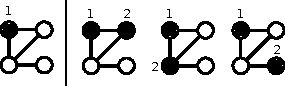
\includegraphics[scale=1.5]{labelling_ext_example.pdf}
    \caption{All possible label extensions of a flag}
    \label{fig:labelling_ext_example}
\end{figure}

The other technicality we need to address is that of the hereditary nature of graph
classes. In the classic flag algebra we always assumed that $\Gcl$ was hereditary. We want
to be able to talk about some non-hereditary graph classes $\Gcl$. This is not a major
obstacle but means we need to adjust our notation.

\begin{definition}[Hereditary Closure]
    Given a graph class $\Gcl$ we define the \textbf{hereditary closure} of $\Gcl$ to be
    the smallest graph class which contains $\Gcl$ and is closed under taking
    induced subgraphs. i.e. it's the graphs $G\in\Gcl$ with their induced subgraphs.

    We denote this as $\HeredG$.
\end{definition}

Now we are ready to define our local flags:

\begin{definition}[Local $\sigma$-Flag]
    Fix some graph class $\Gcl$ and takes its hereditary closure $\HeredG$.
    Let $\sigma$ be a type. Then a $\sigma$-flag $(F, \theta)\in\HeredG{}^\sigma$ is a
    \textbf{local $\sigma$-flag} if we have the following properties:
    \begin{enumerate}
        \item $(G,\eta) \to \rho((F,\theta); (G,\eta))$ is a bounded function as a function
            $\Gcl^\sigma\to\R_{\geq 0}$. (We are very intentionally using $\Gcl$ and not its closure here).
        \item If we label any of $F$'s unlabelled vertices we get another local flag.
    \end{enumerate}
\end{definition}

To state this 2nd property more precisely: We require that for any label extension
$\theta'$ of $\theta$, the induced extended flag $(F,\theta')$ is also a local flag.
This is not a circular definition as any label extension of $(F,\theta)$ reduces the number of
unlabelled vertices
by 1; We could define inductively starting with those flags with no unlabelled vertices.

What we're trying to capture here is that any "subflag"
of $F$ is also a local flag, meaning we can pin down
$F$'s vertices and continue to get bounded behaviour.

\begin{example}
    As in the example above $F=\edgemarked$ gives rise to a bounded local
    density function $\rho$. The only label extension of $F$ is the edge
    with both vertices labelled $F' = \edgebothmarked$. This (as with all flags with no
    unlabelled vertices) has $c(F'; G) = 1$ so $\rho(F; G) = 1/\binom{\Delta(G)}{0}=1$
    which is bounded so $F'$ is a local flag. Hence $F=\edgemarked$ is a local flag.
\end{example}

\begin{note}
    This second property we require of local flags is not necessarily implied by
    the first. See TODO.
\end{note}

We write $\Glocn^\sigma\subseteq\HeredG{}^\sigma_n$ for the set of local $\sigma$-flags
of size $n$ up to isomorphism, and $\Gloc^\sigma$ for all local $\sigma$-flags. As usual we
can drop the $\sigma$ superscript if $\sigma=\emptyset$.

Comparing this section to the classic flag algebra case (section \ref{sec:flag_algebras})
you might expect us to introduce something akin to the chain rule (lemma \ref{lemma:chain_rule}).
Unfortunately no such relation exists in general for local flags. This is the first big
loss when moving to the new framework: Prima facie it's unclear how one can "project"
small flags into the space of larger flags.
